\documentclass[pre,twocolumn,superscriptaddress,amsmath,amssymb,floatfix]{revtex4-2}
\usepackage{graphicx}
\usepackage{booktabs}
\usepackage[colorlinks=true,allcolors=blue]{hyperref}

\begin{document}

\title{Scale-rich network metamaterials grow by local rules on a recursive cell division}

\author{Alexei Vazquez}
\email{alexei@nodeslinks.com}
\affiliation{Nodes \& Links Ltd, Salisbury House, Station Road, Cambridge, CB1 2LA, UK}

\date{\today}

\begin{abstract}
Scale-rich (SR) metamaterials are planar ligament networks grown by nucleating a
segment at a random point and angle and extending it until it meets the existing
structure, with a thickness that decays with the time of birth. In the dual graph,
where ligaments are nodes and junctions are links, the degree distribution has a
$k^{-3}$ tail that was attributed to a spatial preferential attachment. Here we show
that, at zero thickness, the SR construction is Cowan's iterated division of cells
with area-weighted selection, and that its dual graph grows by a face-local rule: a
new node joins the two nodes that carry the sides of one face. Three exact
statements follow. The area fractions of the two daughter cells are uniform, so the
cell hierarchy is a random binary search tree and the cell areas are uniform
spacings. A new ligament ends on a ligament born at $h=tU^2$, with $U$ uniform, so the
thickness ratio between a ligament and its host does not depend on time. The degree of
an interior ligament equals its number of face incidences, which yields linear
preferential attachment and the Barab\'asi--Albert distribution
$p_k=12/[k(k+1)(k+2)]$. Using integral geometry we compute the probability that a
new ligament cuts off a corner of its cell ($2\ln2/\pi$ for a square, $0.448$
averaged over cells), which sets the clustering spectrum
$C(k)\simeq2[p_0+p(k-2)]/[k(k-1)]$. A purely topological face-splitting rule
reproduces $P(k)$, $C(k)$ and $k_{nn}(k)$ but not distances; the half of the
splits that close squares boosts the shortest-path multiplicity above the
configuration-model value. The exponent $\gamma=3$ is pinned by the ratio of links
received to face incidences created; thickness, jamming, angle sets, alignment and
density gradients do not move it, whereas coherent orientation fields
($\gamma\simeq2.4$--$2.5$ up to $T=10^6$) and three-dimensional plates
($\gamma\simeq2.5$) do. At fixed decay exponent, the reported per-ligament energy law
cannot distinguish degree from length or age.
\end{abstract}

\maketitle

%======================================================================
\section{Introduction}

Both \textit{et al.}~\cite{both2026} introduced scale-rich (SR) mechanical
metamaterials, two-dimensional ligament networks in which length, thickness and
connectivity span orders of magnitude. The construction has two parameters. At step
$t=1,2,\dots,T$ a point is drawn uniformly in the unit square together with a uniform
angle, and a ligament of thickness $\lambda_t=\lambda_0t^{-\alpha}$ is grown both ways
from it until each end meets an existing ligament or the boundary. Every junction is a
T. Following the road-network convention~\cite{rosvall2005,kalapala2006}, the authors
represent each ligament as a node and each junction as a link. They report power-law
distributions of thickness, length and degree, with $P(k)\sim k^{-3}$ attributed to a
spatial preferential attachment, because longer ligaments offer more opportunities to
be hit. They also report a per-ligament elastic energy law
$U_i\sim k_i^{3/2}\lambda_i^{1/2}f(\theta_i)$ and a density scaling of the total
energy controlled by $\alpha$~\cite{both2026}.

Two questions are natural from the point of view of network growth. Which growth
class does the SR dual graph belong to, and which of its properties are fixed by
that class rather than by the design parameters $(\alpha,\lambda_0)$? Local growth
rules, in which a new node attaches to an existing node and to some of its
neighbours, generate preferential attachment without global information, together
with a hierarchical clustering spectrum $C(k)\sim1/k$ and degree
correlations~\cite{vazquez2003,holme2002,dorogovtsev2001,ravasz2003}. Here we show
that the SR construction is of this type. The geometric construction is itself not
new: with zero thickness it is Cowan's iterated cell division~\cite{cowan2010}, a
member of the family of random tessellations that also contains the STIT
model~\cite{nagel2005,redenbach2025}. Keeping both references in view, the recursive
division and the local graph rule, turns most of the reported network statistics into
exact or asymptotically exact statements.

The paper is organised as follows. Section~\ref{sec:model} maps the SR construction
onto Cowan's division and derives the statistics of the cell hierarchy. In
Sec.~\ref{sec:degree} we write the dual growth as a face-local rule and obtain its
degree distribution. Section~\ref{sec:triangles} computes the corner-cut probability
by integral geometry and derives the clustering spectrum. Section~\ref{sec:topology}
asks which properties survive when geometry is removed, and Sec.~\ref{sec:paths}
turns to distances and shortest-path multiplicity. Section~\ref{sec:gamma} identifies
which rules move the degree exponent, and Sec.~\ref{sec:energy} discusses what this
means for the reported structure--property relations.

\begin{figure*}[tbp]
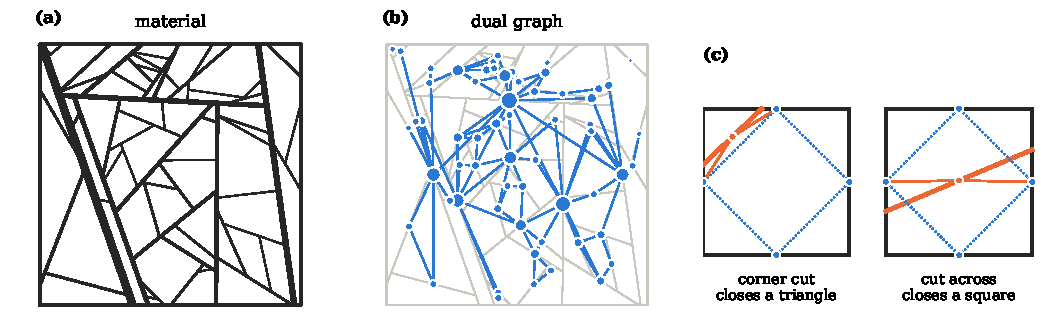
\includegraphics[width=\textwidth]{figs/fig1.pdf}
\caption{(a) An SR realisation with $T=60$ ligaments. The line width increases with
$\lambda_t=\lambda_0t^{-1/2}$. (b) Its dual graph: each ligament is a node, placed
at the ligament midpoint with a size that grows with its degree, and each junction is
a link. (c) A new ligament (orange) splits one cell. Dual nodes of the cell's sides
are shown in blue, and the dotted lines join sides that meet at a corner. If the new
ligament cuts off a corner, it joins two adjacent sides and closes a triangle in the
dual. Otherwise it joins two sides at distance two and closes a square.}
\label{fig:model}
\end{figure*}

%======================================================================
\section{The SR construction is a recursive cell division}
\label{sec:model}

We first set $\lambda_0=0$ and return to thickness at the end of this section. The
current ligaments partition the square into convex polygonal cells. A uniform
point falls in cell $K$ with probability equal to its area $A_K$. Because $K$ is
convex and bounded by ligaments, the new ligament grown from that point stops on the
boundary of $K$: it is the chord of $K$ through a uniform point of $K$ at a uniform
angle. The SR model is therefore the iterated division of cells with
\emph{area-weighted selection} and the \emph{chord through a uniform point} division
rule, model~(a) of Fig.~2 in Cowan~\cite{cowan2010}. Cowan's rescaling of the window
does not change the topology. STIT tessellations differ in both rules: cells are
selected by perimeter and cut by isotropic uniform random
lines~\cite{nagel2005,redenbach2025}. Gilbert's model~\cite{gilbert1967}, used as a
reference architecture in Ref.~\cite{both2026}, grows all segments simultaneously and
is a different process.

\paragraph*{Corner numbers.}
A junction placed on the side of a neighbouring cell is a straight angle there, so
the corner number $n$ of a cell is fixed at birth. A chord ending on two sides gives
each daughter the two new corners at its ends, so $n_1+n_2=n+4$. Starting from the
square, after $t$ steps there are $t+1$ cells and $4+4t$ corners, so the mean corner
number is exactly $\langle n\rangle=4$. Measured number fractions for $n=3,\dots,7$
are $0.301,0.452,0.200,0.042,0.005$.

\paragraph*{Uniform splitting and the binary search tree.}
Let $K$ be a convex body, $x$ a uniform point in $K$, and $\theta$ any direction
independent of $x$. For fixed $\theta$, the offset $s$ of the line through $x$ along
the normal direction has density $w(s)/A_K$, where $w(s)$ is the chord length at
offset $s$. The area on one side of the line is $\int_{-\infty}^s w(s')ds'$, so the
area fraction is the cumulative distribution function of $s$ evaluated at $s$. It is
therefore uniform on $(0,1)$, whatever the shape of $K$ and the law of $\theta$.
Combined with area-weighted selection, this has a direct consequence. Label each cell
by the interval of $[0,1]$ that it would occupy if areas were laid on a line. The
sequence of splits is then exactly that of a binary search tree (BST) built from
uniform keys: the key falls in an interval with probability equal to its length and
splits it at the key~\cite{devroye1986}. Hence the cell areas after $T$ steps are the
$T+1$ spacings of $T$ uniform points, $P(TA>x)\to e^{-x}$, which recovers Cowan's
exponential area law~\cite{cowan2010}, and $\sum_KA_K^2=2/(T+2)$. The depth of the split at
step $t$ grows as $2\ln t$, with variance $2\ln t$, and areas never multiscale. Our
simulations give a depth slope $1.983$, a variance slope $1.980$ and $\sum A^2=9.998\times10^{-5}$
at $T=2\times10^4$ against $9.999\times10^{-5}$ [Fig.~\ref{fig:bst}(a,b)]. The
multiscaling of Krapivsky and Ben-Naim~\cite{krapivsky1994} arises with rectangular
cuts and lives in the lengths, not in the areas. Axis-aligned chords reproduce their
width exponents $\gamma(a)=(a-\sqrt{a^2+4})/2$ within $2\%$, while with isotropic
angles the perimeter moments scale as $t^{1-a/2}$, without multiscaling.

\paragraph*{Lengths and the age of the host.}
Cells at time $t$ have linear size $t^{-1/2}$, and the mean length of the ligament
born at $t$ is $\langle\ell_t\rangle\simeq c_\ell t^{-1/2}$ with $c_\ell=1.16$. The total
length grows as $L(t)\simeq c_L\sqrt t$ with $c_L=2c_\ell=2.33$. The first ligament has
$\langle\ell_1\rangle=0.945$, the $\ell_0$ of Ref.~\cite{both2026}. In the mean-field
approximation of Sec.~\ref{sec:degree}, an end of ligament $t$ lands on a ligament
with probability proportional to its length, so the host's birth index $h$ satisfies
$P(h)\simeq\ell_h/L(t)\simeq\tfrac12(ht)^{-1/2}$. Then $P(h\le xt)=\sqrt x$, that is
\begin{equation}
  h/t\;\to\;U^2,\qquad U\sim\mathrm{Uniform}(0,1).
  \label{eq:host}
\end{equation}
Equivalently, $\ln(t/h)$ is exponential with mean $2$ [Fig.~\ref{fig:bst}(c)].
Measured values of $\langle(h/t)^\alpha\rangle$ are $0.667$, $0.498$ and $0.330$ for
$\alpha=1/4$, $1/2$ and $1$, against $1/(1+2\alpha)=0.667$, $0.500$ and $0.333$.

\paragraph*{Thickness.}
With $\lambda_t=\lambda_0t^{-\alpha}$, Eq.~\eqref{eq:host} gives the thickness ratio
between a new ligament and its host as $\lambda_t/\lambda_h=U^{2\alpha}$. Its law does
not depend on $t$, so every generation couples to the frame it attaches to in the same
statistical way. Its moments $\langle(\lambda_h/\lambda_t)^p\rangle=1/(1-2p\alpha)$
diverge at $\alpha=1/(2p)$; for the bending stiffness of the host ($p=3$) this happens
at $\alpha=1/6$. The fill fraction without overlaps is
$\rho\simeq\lambda_0\sum_t\ell_tt^{-\alpha}\simeq\lambda_0c_\ell\sum_tt^{-\alpha-1/2}$,
which converges only for $\alpha>1/2$. This recovers the boundary between the jammed and
tunable-density phases of Ref.~\cite{both2026}, and $\rho\simeq\lambda_0c_\ell\zeta(\alpha+1/2)$
matches their $\rho\approx\ell_0\lambda_0\zeta(\alpha+\beta)$ with $\beta=1/2$. Thickness
removes area and eventually stops growth in the jammed phase, but it does not change
the rule by which cells are split (Sec.~\ref{sec:gamma}). In what follows the network is
the zero-thickness one unless stated otherwise.

\begin{figure*}[tbp]
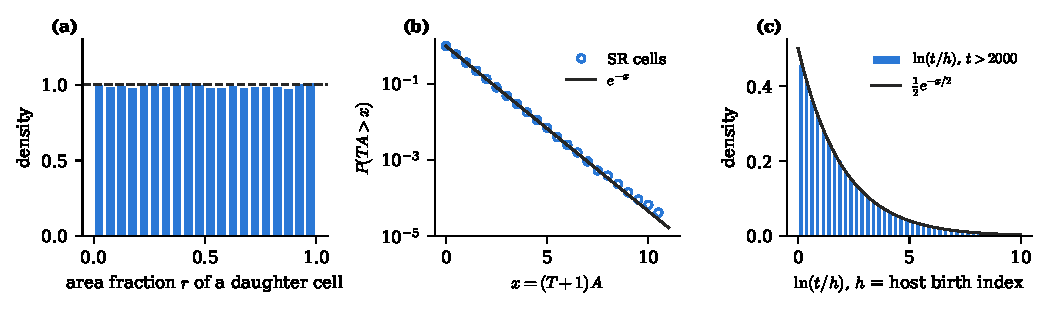
\includegraphics[width=\textwidth]{figs/fig2.pdf}
\caption{The cell hierarchy of the SR construction (six realisations, $T=2\times10^4$).
(a) The area fraction of a daughter cell is uniform. (b) Rescaled cell areas follow
$e^{-x}$, the spacing law of uniform points. (c) The birth index $h$ of the ligament
hit by a new ligament $t$ satisfies $h/t\to U^2$, so $\ln(t/h)$ has density
$\frac12e^{-x/2}$.}
\label{fig:bst}
\end{figure*}

%======================================================================
\section{A face-local growth rule and its degree distribution}
\label{sec:degree}

In the dual graph, step $t$ reads as follows: choose a face (a cell) with probability
equal to its area, choose the two sides of that face that the chord meets, and join
the new node $t$ to the two ligaments that carry them [Fig.~\ref{fig:model}(c)]. The new
node never links to a node outside the chosen face. It is a local rule in the sense of
Ref.~\cite{vazquez2003}, with faces in place of neighbourhoods.

\paragraph*{Incidences equal degree.}
Call an incidence a pair (ligament $i$, cell $K$) in which $i$ contributes a side to
$K$. A new ligament has two incidences, one on each side, and two links. When a later
ligament ends on $i$, it adds one link to $i$ and cuts one of $i$'s sides in two, adding
one incidence. For a ligament whose ends are both interior, the number of incidences
therefore equals the degree $k_i$ at all times. Each step creates two hits and four
incidences, so the total number of incidences is $4t$, in agreement with
$\langle n\rangle=4$.

\paragraph*{Rate equation.}
If every incidence is equally likely to be hit, the rate at which node $i$ gains links
is $2k_i/4t$, linear preferential attachment with
\begin{equation}
  \frac{dk_i}{dt}=\frac{k_i}{2t},\qquad k_i(t)=2\sqrt{t/i}.
  \label{eq:pa}
\end{equation}
This is the Barab\'asi--Albert rule with $m=2$~\cite{barabasi1999}. The master
equation~\cite{krapivsky2001,dorogovtsev2002} gives
\begin{equation}
  p_k=\frac{12}{k(k+1)(k+2)},\qquad P(k'\ge k)=\frac{6}{k(k+1)},
  \label{eq:pk}
\end{equation}
for $k\ge2$, so $\gamma=3$. At $T=10^5$ the measured $K^2P(k-2\ge K)$ at $K=8,16,32$ is
$3.53,4.45,5.19$, against $3.49,4.49,5.16$ from Eq.~\eqref{eq:pk} [Fig.~\ref{fig:degree}(a)].
The degree of the cohort born at $i$ decays as $i^{-\beta}$ with $\beta=0.50$--$0.51$.

\paragraph*{Metric form.}
The spatial preferential attachment of Ref.~\cite{both2026} is the same statement in
metric form. Two ends land per step on a total length $L(t)=c_L\sqrt t$, so the hit
rate per unit length is $2/L(t)$ and
\begin{equation}
  k_i-2=\frac{4\ell_i}{c_L}\left(\sqrt T-\sqrt i\right).
  \label{eq:kl}
\end{equation}
The ratio of measured to predicted degree averages $1.006$, with correlation $0.95$
[Fig.~\ref{fig:degree}(b)]. Equations~\eqref{eq:pa} and \eqref{eq:kl} agree on average
because $\langle\ell_i\rangle=c_\ell i^{-1/2}$ and $4c_\ell/c_L=2$. They differ in
where the randomness sits. In Eq.~\eqref{eq:pa} it is in the history of hits. In
Eq.~\eqref{eq:kl} it is in the birth length, $x=\ell_i/\langle\ell_i\rangle$, with
$\langle x^2\rangle=1.39$. With $k\simeq2x\sqrt{T/i}$ and $i$ uniform, the tail amplitude
is $K^2P(k\ge K)\to4\langle x^2\rangle=5.56$, about $7\%$ below the value $6$ of
Eq.~\eqref{eq:pk}. A hub is therefore predictable at birth from its length, which is
not the case in the Barab\'asi--Albert model.

\begin{figure}[t]
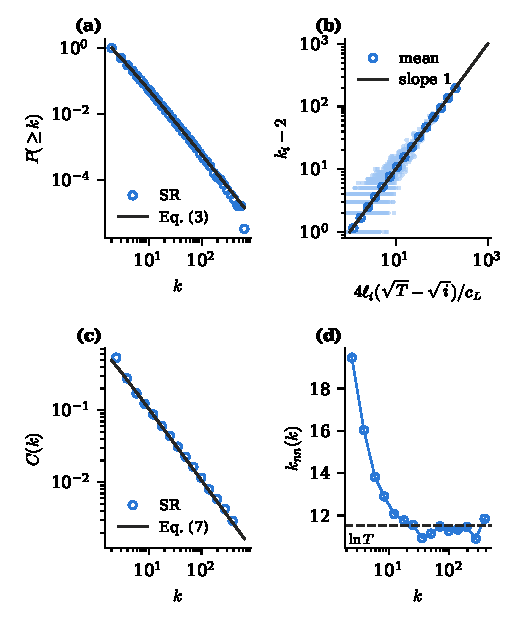
\includegraphics[width=\columnwidth]{figs/fig3.pdf}
\caption{Dual graph of the SR construction, three realisations with $T=10^5$.
(a) Cumulative degree distribution and Eq.~\eqref{eq:pk}. (b) Degree against the
prediction~\eqref{eq:kl} from birth length and age (light dots: a random sample of
ligaments; circles: binned means). (c) Clustering spectrum and
Eq.~\eqref{eq:ck} with $p_0=0.494$, $p=0.53$. (d) Mean neighbour degree; the dashed line
is $\ln T$.}
\label{fig:degree}
\end{figure}

%======================================================================
\section{Corner cuts, triangles and clustering}
\label{sec:triangles}

A new node closes a triangle in the dual when the two ligaments it joins are already
linked. Locally this happens when the chord cuts off a single corner of its cell,
since the two sides meeting at that corner belong to linked ligaments.

\paragraph*{Integral-geometry formula.}
Chords through a uniform point at a uniform angle sample lines with density
$w(s)\,ds\,d\theta/(\pi A_K)$. For a fixed direction $\theta$, order the corners by
their projection on the normal. The chord cuts off the lowest corner alone when its
offset lies between the projections of the lowest and second-lowest corners. The
integral of $w(s)$ over that range is the area $A_{\rm lo}(\theta)$ cut off by the line
through the second-lowest corner, and likewise $A_{\rm hi}(\theta)$ at the other end.
Hence
\begin{equation}
  P_{\rm corner}(K)=\frac{1}{\pi A_K}\int_0^\pi\big[A_{\rm lo}(\theta)+A_{\rm hi}(\theta)\big]\,d\theta .
  \label{eq:corner}
\end{equation}
For a triangle every chord cuts off a corner, so $P_{\rm corner}=1$. For a square,
Eq.~\eqref{eq:corner} gives $2\ln2/\pi=0.4413$, for a $1\times4$ rectangle $0.303$, for
regular pentagons and hexagons $0.232$ and $0.136$~\cite{santalo1976}. Averaged over the
SR cell population, by corner number $n=3,\dots,7$, the values are
$1.000$, $0.461$, $0.254$, $0.152$ and $0.10$, and the area-weighted average is
$0.447$--$0.449$. The measured frequency of corner cuts is $0.447$--$0.449$.

\paragraph*{Triangle bookkeeping.}
A corner cut creates a triangular daughter unless the parent was already a
triangle, which can only split into $(3,4)$. The number fraction of triangles is
therefore $f_3=\langle P_{\rm corner}\rangle-w_3$, where $w_3$ is the area fraction of
triangles. Measured values are $0.30=0.449-0.147$.

\paragraph*{Non-local closures.}
The fraction of new nodes that close a triangle is $0.496$, not $1/2$. Corner cuts
account for $0.448$. The other $0.048$ join two non-adjacent sides of their cell whose
ligaments already meet outside it. The remaining half of the new nodes close a square
around the cell.

\paragraph*{Clustering spectrum.}
Links between existing nodes are never added. A node therefore acquires triangles only
at birth, with probability $p_0$, or when it is hit and the other end of the new
ligament lands on one of its neighbours, with probability $p$ per hit. The number of
triangles at node $i$ is $e_i=p_0+p(k_i-2)$, and
\begin{equation}
  C(k)=\frac{2[p_0+p(k-2)]}{k(k-1)}\simeq\frac{2p}{k},
  \label{eq:ck}
\end{equation}
the hierarchical form produced by triadic
closure~\cite{vazquez2003,ravasz2003,holme2002}. With $p_0=0.494$ and a fitted $p=0.53$,
Eq.~\eqref{eq:ck} is within $2\%$ of the data for $k\ge15$ [Fig.~\ref{fig:degree}(c)].
The mean clustering is $0.38$. At $k=2$ the measured $C=0.536$ exceeds $p_0$, because
corner-cut ligaments are short and rarely hit again. The degree assortativity is
$r\simeq-0.02$. The mean neighbour degree $k_{nn}(k)$ falls from $19.5$ at $k=2$ to a
plateau of $11.1$--$11.5$ for hubs, close to the Barab\'asi--Albert value
$(m/2)\ln T=\ln T=11.5$ [Fig.~\ref{fig:degree}(d)].

In the language of local rules, the SR dual mixes two moves. With probability $\simeq0.45$
the new node attaches to both ends of a link (the corner), as in the edge-attachment
model of Dorogovtsev, Mendes and Samukhin~\cite{dorogovtsev2001}, except that the
link is selected with probability proportional to the area of its cell rather than
uniformly. With probability $\simeq0.55$ it attaches to two nodes at distance two on a
face cycle and closes a square. The edge-attachment model has $\gamma=3$ and
clustering $0.74$~\cite{dorogovtsev2001,dorogovtsevgoltsev2002}. The SR dual has the
same $\gamma$ and half the clustering; the other half of the closures went into squares.
It is also the two-dimensional relative of the random Apollonian
network~\cite{andrade2005,zhou2005}, in which faces are selected and a node's degree is
proportional to the number of faces it bounds.

%======================================================================
\section{What topology alone reproduces}
\label{sec:topology}

To separate the role of geometry, we grew a purely topological surrogate. Each face is
stored as a cyclic list of the nodes that carry its sides. At each step a face is chosen
uniformly. If it is a triangle, two of its sides are joined; otherwise two adjacent
sides are joined with probability $p_4$, or two non-adjacent sides with probability
$1-p_4$. The face is then split into two, with $n_1+n_2=n+4$ as in the tessellation.
No lengths or positions are used.

Every face-local variant we tried (faces chosen uniformly, by number of sides, or by
a random-split area) reproduces Eq.~\eqref{eq:pk}: $\gamma_{\rm MLE}(k\ge10)=2.88$--$2.91$
and the same $K^2P$ amplitudes. The single parameter $p_4=0.29$ also gives a mean
clustering of $0.386$ (SR, $0.377$) and places $C(k)$ and $k_{nn}(k)$ on the SR curves.
A variant in which sides are chosen with probability proportional to a mean-field
length, instead of uniformly, breaks the equality between hits and incidences and gives
$\gamma\simeq3.6$. The degree statistics are therefore fixed by the face-local rule and
by the equivalence of incidences, not by the geometry.

The surrogate fails on distances. At $T=10^5$ its mean distance is $14.1$ against $8.8$
for SR, and it grows as $1.43\ln T$ against $0.60\ln T$ [Fig.~\ref{fig:paths}(a)].
Faces cut across, in the surrogate, stack into long ladders of squares. In the geometric
model chords hit long sides preferentially, and long sides belong to old, long
ligaments, so new nodes stay close to the hubs and the dual remains small-world.
Geometry matters for metric properties only.

\begin{figure*}[tbp]
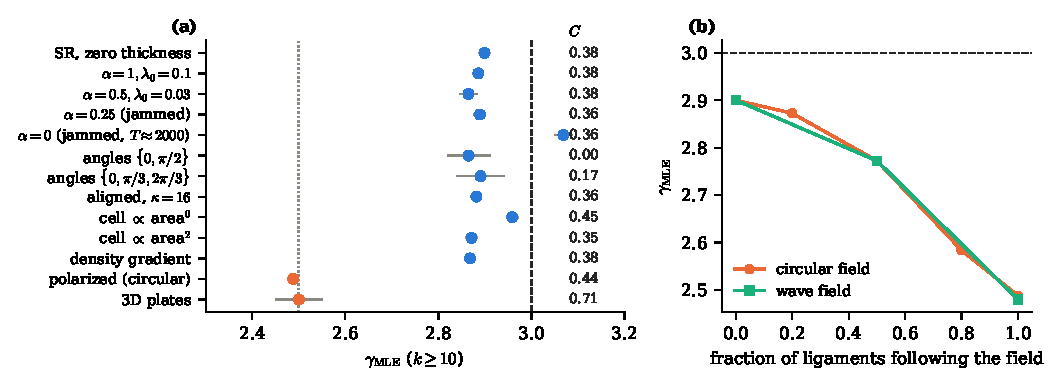
\includegraphics[width=\textwidth]{figs/fig4.pdf}
\caption{(a) Maximum-likelihood exponent ($k\ge10$) for the design rules of
Ref.~\cite{both2026}, $T=3\times10^4$, two realisations (the jammed $\alpha=0$ case stops at
$T\simeq2000$; 3D plates at $T=8\times10^4$, $k\ge40$). The number on the right is the mean
clustering coefficient. Dashed line: $\gamma=3$; dotted line: $\gamma=2.5$.
(b) Exponent against the fraction of ligaments whose angle follows a circular or a wave
orientation field ($T=3\times10^4$); the remaining ligaments have uniform angles.}
\label{fig:gamma}
\end{figure*}

%======================================================================
\section{Fewest-turn paths and their multiplicity}
\label{sec:paths}

A shortest path in the dual graph is a route through the material that changes
ligament the fewest times. For a random graph with given degrees, the mean number of
shortest paths between two nodes is $\langle\mu\rangle\simeq c_2/e$ with
$c_2=\langle k(k-1)\rangle/\langle k\rangle$, and local growth rules depart from this
value in a rule-dependent way~\cite{vazquezpaths2026}. For $\gamma=3$, $c_2$ grows as
$\ln T$; we measure $c_2=7.9$ at $T=10^3$ and $15.6$ at $T=3\times10^5$.

The degree-preserving randomisation of the SR dual follows the configuration-model
value, with $\langle\mu\rangle/(c_2/e)=1.03$, $0.98$, $0.95$, $0.94$ and $0.89$ for
$T=10^3,\dots,10^5$. The SR dual itself exceeds it by a factor that grows with size:
$2.3$, $2.8$, $3.9$, $4.9$, $4.9$ and $6.8$ for $T=10^3,\dots,3\times10^5$. The
edge-attachment model stays close to the baseline ($0.9$--$1.2$) over the same range,
so triangles add no redundancy. The excess comes from the square-closing half of the
splits: the number of shortest paths grows with distance at a rate of $0.45$--$0.6$
per hop, as on a square lattice, where fewest-turn routes through a grid of ligaments
are many. Because $\mu$ has a heavy tail, Fig.~\ref{fig:paths}(b) shows
$\langle\ln\mu\rangle$, which grows as $0.18\ln T$ for SR against $0.06\ln T$ for the
randomised graph. In the surrogate the ladders make the multiplicity explode
($\langle\ln\mu\rangle=3.4$ at $T=3\times10^5$). The squares supply the redundancy,
while the geometry keeps them from stacking.

\begin{figure}[t]
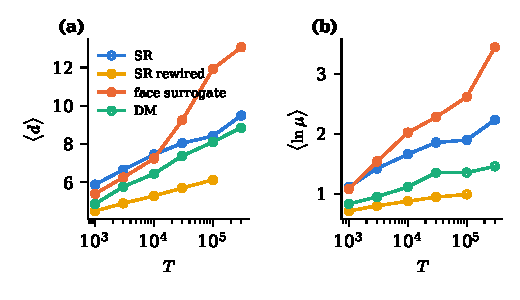
\includegraphics[width=\columnwidth]{figs/fig5.pdf}
\caption{(a) Mean distance in the dual graph against $T$ for the SR construction, its
degree-preserving randomisation, the topological face surrogate ($p_4=0.29$) and the
edge-attachment (DM) model~\cite{dorogovtsev2001}. (b) Mean logarithm of the
shortest-path multiplicity. Averages over three realisations and 100 sources.}
\label{fig:paths}
\end{figure}

%======================================================================
\section{What moves the degree exponent}
\label{sec:gamma}

In a growth rule where each new node creates a fixed number of incidences and old
nodes are hit in proportion to theirs, the exponent is $\gamma=1+1/b$, with $b$ the
number of links received by old nodes per step divided by the number of incidences
created per step. In two dimensions every new ligament makes two junctions and four
incidences, so $b=1/2$ and $\gamma=3$, whatever the cell selection, the angle and the
thickness, provided the hit rate per incidence is uniform across nodes.

We tested this with the design rules of Ref.~\cite{both2026} at $T=3\times10^4$, two
realisations each [Fig.~\ref{fig:gamma}(a)]:
\begin{itemize}
\item Thickness in the tunable-density phase ($\alpha=0.5$--$1$, $\lambda_0=0.01$--$0.1$,
$\rho=0.12$--$0.45$) gives $\gamma_{\rm MLE}=2.85$--$2.92$, $\beta=0.50$--$0.52$,
$C=0.376$--$0.378$, and a triangle closure of $0.49$--$0.50$.
\item In the jammed phase ($\alpha=0$--$0.4$), growth stops when the free area is
exhausted (at $t\simeq2000$ for $\alpha=0$, $\lambda_0=0.02$). Jamming truncates $T$; it
does not change $\gamma$ ($2.89$--$2.94$ wherever the statistics allow) or $C$
($0.35$--$0.37$).
\item Angle sets change clustering but not $\gamma$. With angles $\{0,\pi/2\}$ all cells are
rectangles, so $C=0$ exactly and $\gamma=2.87$; this is the rectangular fragmentation of
Ref.~\cite{krapivsky1994}. With $\{0,\pi/3,2\pi/3\}$, $C=0.17$.
\item Global alignment (von Mises, $\kappa$ up to $16$), cell selection proportional to
area$^q$ ($q=0,0.5,2$), and linear or radial density gradients give $\gamma=2.86$--$2.96$.
Selection with $q=0$ raises $C$ to $0.45$, and $q=2$ lowers it to $0.35$.
\end{itemize}
The angle set and the selection weight therefore tune clustering between $0$ and $0.45$,
while the exponent stays at $3$.

\paragraph*{Coherent orientation fields.}
The polarized rule of Ref.~\cite{both2026}, in which the angle follows a prescribed
field $\theta(x,y)$, breaks the uniformity of the hit rate. Locally parallel newcomers
cannot hit each other; they end on the ligaments that are misaligned with the local field,
and for straight ligaments in a curved field the misalignment grows with length. The
degree then grows faster than length, $k\sim\ell^{1.5\text{--}1.6}$ instead of
$\ell^{1.03}$. For a circular field and for waves $\theta=\pi(x+y)/w$ with
$w=0.125$--$1$ we find $\gamma\simeq2.44$--$2.51$ and cohort exponents $\beta\simeq0.6$--$0.67$,
stable from $T=10^4$ to $2\times10^5$. At $T=10^6$ the maximum-likelihood exponent is
$2.43$--$2.50$ ($k\ge10$ to $k\ge40$) for the circular field and $2.36$--$2.47$ for the
shortest wave ($w=0.125$), while the uniform control gives $2.88$--$2.98$, so the effect
does not wash out at this size. The exponent decreases continuously as the fraction of
ligaments following the field increases [Fig.~\ref{fig:gamma}(b)].

\paragraph*{Three dimensions.}
For plates in a cube, a new plate meets $\bar m$ existing plates (the sides of its
section polygon), creates $2+\bar m$ incidences and hands out $\bar m$ links. Then
$b=\bar m/(2+\bar m)$ and $\gamma=2+2/\bar m$. We measure $\bar m=4.47$--$4.57$, which
predicts $\gamma=2.44$. The dimensional argument $k\sim(\ell/\ell_T)^{d-1}$ gives
$\gamma=(2d-1)/(d-1)=2.5$, the exponent of random Apollonian networks in $d$
dimensions~\cite{kolossvary2016}. At $T=8\times10^4$ the measured value is $2.50$
($k\ge40$), with $\beta=0.66$. Three-dimensional SR materials therefore have
$\gamma\simeq2.5$, not $3$.


%======================================================================
\section{Consequences for structure--property relations}
\label{sec:energy}

At fixed $\alpha$, the thickness of ligament $i$ is $\lambda_0i^{-\alpha}$ exactly,
and its degree and length both scale as $i^{-1/2}$ on average
[Eqs.~\eqref{eq:pa} and \eqref{eq:kl}]. The marginal laws reported in
Ref.~\cite{both2026}, an energy that decays as $i^{-(3/4+\alpha/2)}$ with the
introduction time and the corresponding powers of $k$, $\ell$ and $\lambda$, are one
age law written in different variables. A product $U\sim k^a\lambda^b$ reproduces the
age law for every $\alpha$ only if $a/2+\alpha b=3/4+\alpha/2$, that is $a=3/2$ and
$b=1/2$, the reported exponents. Because $k\propto\ell$ at fixed age
[Eq.~\eqref{eq:kl}], the same data are described equally well by
$U\sim\ell^{3/2}\lambda^{1/2}f(\theta)$. Degree, length and age cannot be separated
from cohort scaling alone.

As an illustration, we computed per-ligament energies in an Euler--Bernoulli frame
(axial area $\lambda$, bending moment of inertia $\lambda^3/12$, rigid T-junctions,
affine uniaxial strain on the boundary) for $T=1000$--$5000$. Fits on degree and on
length are indistinguishable, $U\propto k^{1.64}\lambda^{1.61}$ ($R^2=0.634$) against
$U\propto\ell^{0.82}\lambda^{2.02}$ ($R^2=0.631$), and the age alone gives an $R^2$
within $0.03$--$0.08$ of the best fit. Within a birth cohort the partial correlations
of $U$ with $k$ ($0.22$--$0.30$) and with $\ell$ ($0.17$--$0.34$) are comparable. The thickness
exponent of a slender-beam frame lies between stretching ($1$) and bending ($3$) and is
not $1/2$. A frame of slender beams is not the continuum finite-element model of
Ref.~\cite{both2026}, so we do not attach weight to this exponent. The identifiability
statement does not depend on it.

The same reasoning applies to design. Thickness is a function of birth order, and
degree and length are statistically slaved to birth order, so $\alpha$ and $\lambda_0$
act on the material through the age of each ligament on a fixed network. Connectivity
becomes a design variable only when the growth rule is changed so that $b$ moves away
from $1/2$, as with coherent orientation fields or in three dimensions.

%======================================================================
\section{Discussion}

The scale-rich construction joins two known structures. Geometrically it is Cowan's
recursive division of cells~\cite{cowan2010}; as a graph it is a face-local growth
rule~\cite{vazquez2003} whose degree distribution is the Barab\'asi--Albert form with
$m=2$. The recursion explains the cell hierarchy: uniform split fractions, a
binary-search-tree genealogy and exponential areas. The local rule explains the
network: linear preferential attachment from the identity between degree and face
incidences, a hierarchical clustering spectrum from corner cuts, and an excess of
shortest paths from square-closing splits. Keeping both references in view settles which
features are fixed by the class and which can be designed. The exponent $\gamma=3$, the
equality $\langle n\rangle=4$, the host-age law $h/t\to U^2$ and the stationarity of the
thickness ratio are fixed. Clustering is designable through the angle set and the
selection weight. The degree exponent is designable only through rules that change $b$.

Several points remain open. The uniformity of the hit rate per incidence is a mean-field
assumption, accurate to a few per cent in the tail but not proven. The per-hit triangle
probability $p\simeq0.53$ and the non-local closure fraction $0.048$ require the joint
law of cell shapes next to long ligaments. Under coherent orientation fields we observe
$\gamma\simeq2.4$--$2.5$ up to $T=10^6$ but have no theory of its value. In three
dimensions the two estimates, $2.44$ and $2.5$, are not separated by our data. Finally,
the growth of the shortest-path multiplicity with $T$ is consistent with both a
log-quadratic and a weak power law over the range studied.

More broadly, the SR dual is a reminder that a spatial growth process can carry a
non-spatial growth class. Here the area-weighted point and the convexity of the cells do
the work of a random walk on the graph: they deliver the new node to a face, and the face
does the rest.

\begin{acknowledgments}
All code is available at \url{https://github.com/av2atgh/scalerich}.
The calculations were assisted by Claude Opus~5, an AI assistant developed by Anthropic. Nodes \& Links Ltd
provided support in the form of salary for Alexei Vazquez but did not have any additional role in the conceptualization of the study, the
analysis, the decision to publish or the preparation of the manuscript.
\end{acknowledgments}

\bibliography{references}

\end{document}
